\chapter{Identifikasi Masalah dan Rancangan Solusi}

Bab Identifikasi Masalah dan Rancangan Solusi berisi tentang penjelasan analisis permasalahan yang menjadi dasar dari tugas akhir ini. Secara garis besar, proses perancangan solusi akan mengikuti metodologi yang sudah ditetapkan yaitu pendekatan \textit{User-Centered Design} (UCD) menurut ISO 9241-210. Proses yang akan dibahas pada bab ini meliputi perancangan proses desain, identifikasi konteks penggunaan, analisis kebutuhan perangkat lunak, dan perancangan prototipe perangkat lunak. Gambaran alur UCD yang digunakan pada tugas akhir dapat dilihat pada Gambar \ref{fig:diagram_alur_kerja}.

\begin{figure}[h]
  \centering
  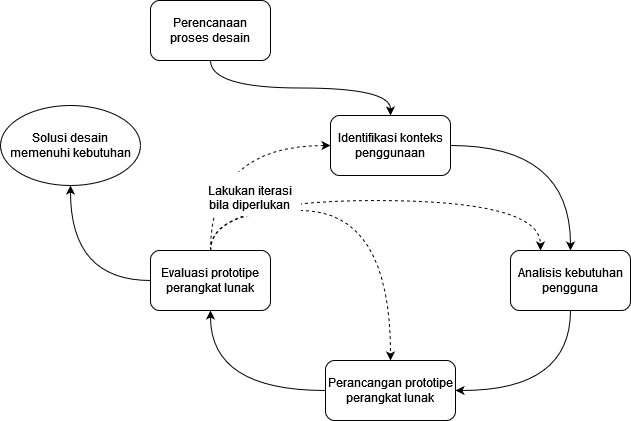
\includegraphics[width=0.8\textwidth]{chapter-1-method.png}
  \caption{Alur Kerja Penelitian}
  \label{fig:diagram_alur_kerja}
\end{figure}

\section{Perancangan Proses Desain}
\label{sec:perancangan_proses_desain}

Pada tahap perancangan proses desain dilakukan persiapan sumber daya yang diperlukan selama proses desain, serta penentuan ruang lingkup permasalahan.

Adapun ruang lingkup permasalahan yang ditentukan selama pengerjaan tugas akhir sebagai berikut

\begin{enumerate}
  \item Target Pengguna
  \subitem Target pengguna selama penelitian adalah pengguna \textit{smartphone} berbasis Android di Indonesia dengan rentang umur 18-34 tahun. Rentang usia tersebut adalah usia mayoritas pengguna media sosial di Indonesia. \parencite{mediasosial2020} 
  
  \item Fungsionalitas Aplikasi
  \subitem Lingkup fungsionalitas aplikasi adalah bagaimana desain interaksi yang baru dapat memperbaiki masalah yang ditemukan pada aplikasi Digital Wellbeing saat ini. Fungsionalitas dar aplikasi menyesuaikan dengan analisis hasil yang didapatkan dari riset dan wawancara. 
   
  \item Lingkup Pengembangan Aplikasi
  \subitem Desain interaksi aplikasi pencegah distraksi yang dibuat memiliki bentuk \textit{mobile interface} dengan mewujudkan sebuah prototipe aplikasi dalam \textit{platform Android}. Aplikasi Digital Wellbeing milik Google ditetapkan menjadi garis dasar pengembangan prototipe aplikasi tersebut.

\end{enumerate}

\section{Identifikasi Konteks Penggunaan}
\label{sec:identifikasi_konteks_penggunaan}

Pada tahap ini dilakukan proses analisis pengguna melalui data yang didapatkan dari ulasan pengguna aplikasi Digital Wellbeing dari situs Google Play Store, serta riset dengan metode wawancara.
% Hasil analisis pengguna digunakan untuk menyusun kebutuhan fungsional 

\subsection{Riset dan Analisis Pengguna}
\label{subsec:riset_analisis}

Tahap ini bertujuan untuk menganalis target pengguna, sehingga didapatkan data perilaku, masalah, tujuan, dan kebutuhan pengguna aplikasi Digital Wellbeing. Riset dilakukan dengan mengumpulkan data ulasan pengguna aplikasi Digital Wellbeing dari situs Google Play Store \textcite{dwplaystorereviews}. Metode pengumpulan data ini dipilih dengan alasan mengacu pada ISO 9241-210, bahwa informasi yang sudah tersedia dari suatu produk dapat dimanfaatkan untuk melakukan modifikasi atau peningkatan kualitas produk \parencite{iso9241-210:2010}, dalam hal ini informasi berbentuk ulasan pengguna.

Hasil terhadap analisis ulasan pengguna kemudian diverifikasi dengan wawasan yang didapat dari wawancara. Karena pada data ulasan pengguna dari Google Play Store tidak terdapat informasi mengenai umur dan perilaku pengguna, wawancara dengan pengguna yang termasuk ke dalam lingkup permasalahan perlu dilakukan juga untuk mendapatkan wawasan mengenai perilaku pengguna. Perilaku pengguna berguna untuk menyusun persona pengguna.

\subsubsection{Ulasan Pengguna}
\label{subsubsec:ulasan_pengguna}

Berdasarkan situs Google Play Store per 13 April 2022, terdapat 609.005 ulasan untuk aplikasi Digital Wellbeing. Untuk menentukan jumlah \textit{sample size}, ditentukan \textit{confidence level} sebesar 95\%. Dikumpulkan data sebanyak 1000 ulasan dari target pengguna yang telah disebutkan pada bab \ref{sec:identifikasi_konteks_penggunaan},  kemudian dikategorikan secara manual, lalu didapatkan 288 ulasan yang dapat digunakan untuk menyusun masalah pengguna, sehingga \textit{sample} data memiliki \textit{margin of error} sebesar 5.78\%.

Metode pengkategorian ulasan dilakukan secara manual yang menghasilkan 11 kategori. Rincian tentang kategori tersebut dapat dilihat pada tabel \ref{tab:daftar_kategori}.

\RaggedLeft
\begin{small}
\begin{longtable}[c]{|W{c}{0.08\textwidth}|>{\baselineskip=12pt}m{0.72\textwidth}|>{\centering\arraybackslash\baselineskip=12pt}m{0.1\textwidth}|}
  \caption{Daftar Kategori Ulasan}
  \label{tab:daftar_kategori} \\
  \hline \rowcolor[HTML]{A3E5F5} \textbf{ID} & \centering\textbf{Kategori Ulasan} & \textbf{Jumlah Ulasan} \\ \hline \endfirsthead
  \hline \rowcolor[HTML]{A3E5F5} \textbf{ID} & \centering\textbf{Kategori Ulasan} & \textbf{Jumlah Ulasan} \\ \hline \endhead
  
  \hline \endfoot
  
  KU-01    & Kurangnya widget untuk menampilkan data di Home Screen & 63 \\ \hline
  KU-02    & Perlu dikembangkannya fitur laporan penggunaan aplikasi untuk menampilkan data & 47 \\ \hline
  KU-03    & Perlu dikembangkannya fitur Focus Mode untuk membatasi jeda dan menambah keketatan & 47 \\ \hline
  KU-04    & Perlu dikembangkannya kemampuan penjadwalan untuk fitur App Timer dan Focus Mode & 36 \\ \hline
  KU-05    & Kurangnya fitur pengaturan tingkat keketatan untuk fitur-fitur & 29 \\ \hline
  KU-06    & Kurangnya kemampuan penundaan untuk fitur App Timer & 18 \\ \hline
  KU-07    & Perlu dikembangkannya fitur Bedtime Mode untuk membatasi penundaan aktivasi fitur dan membatasi akses terhadap aplikasi & 12 \\ \hline
  KU-08    & Kurangnya penjelasan atau susunan kata yang dapat memotivasi pengguna untuk memakai fitur-fitur aplikasi & 12 \\ \hline
  KU-09    & Kurangnya fitur pengelompokkan aplikasi & 11 \\ \hline
  KU-10    & Kurangnya fitur pengaturan jam untuk akhir sebuah hari & 7 \\ \hline
  KU-11    & Kurangnya fitur \textit{whitelisting} untuk pembatasan akses aplikasi oleh Focus Mode & 6 \\ \hline
\end{longtable}
\end{small}
\justifying

\FloatBarrier

Adapun sejumlah ulasan yang tidak tergolong dalam kategori dinilai tidak relevan dalam penyusunan masalah pengguna, dengan penjelasan sebagai berikut

\begin{enumerate}
  \item Ulasan yang menilai positif aplikasi tanpa menyebutkan adanya masalah yang ditemukan dari aplikasi
  \item Ulasan yang menilai negatif aplikasi tanpa menyebutkan masalah yang ditemukan dari aplikasi
  \item Ulasan yang menyebutkan adanya bug dari aplikasi, seperti tidak berfungsinya sebuah fitur di perangkat tertentu
  \item Ulasan yang menyebutkan masalah yang tidak termasuk ke dalam batasan tugas akhir
  \item Ulasan yang tidak dapat dimengerti, seperti huruf-huruf yang tersusun secara acak 
  \item Ulasan yang melaporkan bahwa aplikasi tidak dapat dihapus dari perangkat
\end{enumerate}

\subsubsection{Perilaku Pengguna}
Setelah melakukan analisis ulasan pengguna untuk aplikasi Digital Wellbeing, dilakukan wawancara untuk mendapatkan perilaku pengguna, memverifikasi masalah pengguna dari analisis ulasan, serta menemukan masalah lain yang tidak ditemukan dari ulasan. Wawancara dilakukan secara \textit{online} karena kondisi pandemi COVID-19 yang masih berlangsung di Indonesia. Target berjumlah 5 orang dengan kriteria berusia 18-34 tahun sebagaimana telah dijelaskan pada subbab \ref{sec:perancangan_proses_desain}. Jumlah tersebut dipilih karena menurut \textcite{nielsenusabilityproblems}, penelitian dengan 5 orang responden sudah cukup untuk menemukan rata-rata 85\% masalah dari desain sebuah produk, dan menambah responden lebih banyak akan mendapatkan wawasan tambahan yang semakin sedikit.

Rancangan pertanyaan dapat dilihat pada Lampiran \ref{chpt:daftar_pertanyaan_wawancara}. Data perilaku serta hasil verifikasi ulasan pengguna yang didapat digunakan dalam analisis masalah, tujuan, dan kebutuhan pengguna. Detail pemetaan pengamatan dengan pertanyaan wawancara dapat dilihat pada Tabel \ref{tab:pemetaan_pengamatan_wawancara}

\RaggedLeft
% \begin{longtable}[l]{|m{0.08\textwidth}|>{\baselineskip=12pt}m{0.72\textwidth}|>{\centering\arraybackslash\baselineskip=12pt}m{0.1\textwidth}|}
\begin{longtable}[c]{|>{\baselineskip=15pt}m{0.68\textwidth}|p{0.22\textwidth}|}
  \caption{Pemetaan Pengamatan dengan Pertanyaan Wawancara}
  \label{tab:pemetaan_pengamatan_wawancara} \\
  \hline \rowcolor[HTML]{A3E5F5} \multicolumn{1}{|c|}{\textbf{Pengamatan}} & \multicolumn{1}{|c|}{\textbf{No. Pertanyaan}} \\ \hline \endfirsthead
  \hline \rowcolor[HTML]{A3E5F5} \multicolumn{1}{|c|}{\textbf{Pengamatan}} & \multicolumn{1}{|c|}{\textbf{No. Pertanyaan}} \\ \hline \endhead

  \hline \endfoot
  
  \rowcolor[HTML]{DCF3FC} \multicolumn{2}{|l|}{\textbf{A. Perilaku Responden}} \\ \hline
  Identitas responden & 1, 2, 3 \\ \hline
  Perilaku penggunaan \textit{smartphone} responden & 4, 5, 6, 7, 8 \\ \hline
  Perilaku Responden Terkait Aplikasi Pencegah Distraksi & 9, 10, 11, 12 \\ \hline
  Perilaku Responden Terkait Aplikasi \textit{Digital Wellbeing} & 13, 14, 15 \\ \hline
  \rowcolor[HTML]{DCF3FC} \multicolumn{2}{|l|}{\textbf{B. Verifikasi Ulasan Aplikasi Digital Wellbeing}} \\ \hline
  Verifikasi masalah kurangnya fitur widget pada Homescreen & 16, 17, 18 \\ \hline
  Verifikasi masalah pada fitur laporan data penggunaan aplikasi pada \textit{smartphone} & 19 \\ \hline
  Verifikasi masalah pada fitur Focus Mode & 20, 21 \\ \hline
  Verifikasi masalah untuk kemampuan penjadwalan pada fitur-fitur & 22, 23, 24 \\ \hline
  Verifikasi masalah kurangnya fitur pengaturan tingkat keketatan & 25, 26, 27 \\ \hline
  Verifikasi masalah kurangnya fitur penundaan pada App Timer & 28, 29, 30 \\ \hline
  Verifikasi masalah pada fitur Bedtime Mode & 31, 32, 33 \\ \hline
  Verifikasi masalah kurangnya penjelasan dan susunan kata & 34, 35 \\ \hline
  Verifikasi masalah kurangnya fitur pengelompokkan aplikasi & 36 \\ \hline
  Verifikasi masalah kurangnya fitur pengaturan jam akhir hari & 37 \\ \hline
  Verifikasi masalah kurangnya kemampuan \textit{whitelisting} & 38 \\ \hline
\end{longtable}
\justifying

\FloatBarrier

Jumlah responden yang didapat adalah 10 (sepuluh) orang. Data hasil wawancara dapat dilihat pada Lampiran \ref{chpt:hasil_wawancara}. Dari 10 responden, ditemukan \{jelasin penemuan\} 

... Keseluruhan data perilaku pengguna dirangkum pada Tabel \ref{tab:perilaku_pengguna}

\RaggedLeft
\begin{longtable}[c]{|W{c}{0.08\textwidth}|>{\baselineskip=12pt}m{0.82\textwidth}|}
  \caption{Daftar Perilaku Pengguna}
  \label{tab:perilaku_pengguna} \\
  \hline \rowcolor[HTML]{A3E5F5} \textbf{ID} & \multicolumn{1}{|c|}{\textbf{Perilaku Pengguna}} \\ \hline \endfirsthead
  \hline \rowcolor[HTML]{A3E5F5} \textbf{ID} & \multicolumn{1}{|c|}{\textbf{Perilaku Pengguna}} \\ \hline \endhead
  
  \hline \endfoot
  
  P-01  &  Perilaku 1 \\ \hline
  P-02  &  Perilaku 2 \\ \hline
  P-03  &  Perilaku 3 \\ \hline
  P-04  &  Perilaku 4 \\ \hline
  P-05  &  Perilaku 5 \\ \hline
\end{longtable}
\justifying

\FloatBarrier

\subsubsection{Masalah Pengguna}
\label{subsubsec:masalah_pengguna}

Ditemukan bahwa kategori ulasan yang didapat dari analisis ulasan pengguna cukup bervariasi dengan jumlah yang tersebar. Selain itu, perilaku pengguna yang dianalisis dari wawancara menemukan bahwa \{jelasin hasil analisis pengguna\}. Keseluruhan kategori ulasan dan perilaku pengguna  kemudian dianalisis dan dirangkum menjadi daftar masalah pengguna yang dapat dilihat pada Tabel \ref{tab:daftar_masalah}.

\FloatBarrier

\RaggedLeft
\begin{longtable}[c]{|W{c}{0.12\textwidth}|>{\baselineskip=12pt}m{0.65\textwidth}|>{\centering\arraybackslash\baselineskip=12pt}m{0.15\textwidth}|}
  \caption{Daftar Masalah Pengguna}
  \label{tab:daftar_masalah} \\
  \hline \rowcolor[HTML]{A3E5F5}
  \textbf{ID} & \centering\textbf{Masalah Pengguna} & \textbf{Kategori} \\ \hline \endfirsthead
  \hline \rowcolor[HTML]{A3E5F5}
  \textbf{ID} & \centering\textbf{Masalah Pengguna} & \textbf{Kategori} \\ \hline \endhead

  \hline \endfoot

  MP-01  & Aplikasi Digital Wellbeing kurang memiliki aksesibilitas pada Homescreen terhadap fitur-fitur utama dan data penggunaan aplikasi melalui widget & KU-01 \\ \hline
  MP-02  & Aplikasi Digital Wellbeing kurang memberikan laporan yang komprehensif tentang aktivitas penggunaan aplikasi-aplikasi pada \textit{smartphone} & KU-02 \\ \hline
  MP-03  & Fitur-fitur pada aplikasi Digital Wellbeing kurang dapat membatasi akses pengguna terhadap aplikasi-aplikasi di \textit{smartphone} dengan cukup ketat & KU-03, KU-04, KU-08 \\ \hline
  MP-04  & Fitur-fitur pada aplikasi Digital Wellbeing kurang memberikan fleksibilitas dalam menunda pembatasan akses pengguna terhadap aplikasi-aplikasi di \textit{smartphone} & KU-03, KU-04, KU-06 \\ \hline
  MP-05  & Aplikasi Digital Wellbeing kurang memberikan fleksibilitas bagi pengguna dalam mengatur jadwal aktivasi fitur-fitur & KU-05, KU-07, KU-10 \\ \hline
  MP-06  & Aplikasi Digital Wellbeing tidak dapat mengelompokkan aplikasi-aplikasi pada \textit{smartphone} berdasarkan kategori yang ditentukan oleh pengguna & KU-9 \\ \hline
  MP-07  & Aplikasi Digital Wellbeing tidak memiliki pilihan untuk melakukan \textit{whitelisting} terhadap akses aplikasi-aplikasi pada \textit{smartphone} & KU-11 \\ \hline
\end{longtable}
\justifying

\FloatBarrier


\subsubsection{Kebutuhan Pengguna}
\label{subsubsec:kebutuhan_pengguna}

% Dari permasalahan yang telah diuraikan pada subbab \ref{sec:analisis_masalah}, terdapat beberapa solusi yang dapat diimplementasikan ke dalam aplikasi pencegah distraksi untuk mencapai tujuan dari aplikasi Digital Wellbeing dengan lebih baik yaitu menghambat akses pengguna terhadap aplikasi distraksi secara efektif dan memotivasi pengguna untuk mengubah pola penggunaan aplikasi secara general. Setiap solusi akan dijelaskan tentang permasalahan apa yang akan diselesaikan. Solusi yang ditawarkan untuk menyelesaikan masalah yang telah dianalisis dicantumkan pada Tabel \ref{tab:daftar_solusi}. Rincian mengenai solusi tersebut dapat dilihat pada Lampiran \ref{chpt:rincian_analisis_solusi}.

Berdasarkan hasil analisis permasalahan yang dilakukan, maka solusi yang akan dibuat adalah sebuah prototipe aplikasi pencegah distraksi dengan tampilan mendekati aplikasi Digital Wellbeing yang dapat menyelesaikan rumusan masalah yang telah disebutkan pada Tabel \ref{tab:daftar_masalah}. Pada Tabel \ref{tab:daftar_kebutuhan} terdapat pemetaan rumusan masalah kepada rancangan solusi dalam bentuk kebutuhan fungsional dan kebutuhan interaksi yang akan dimiliki oleh prototipe aplikasi

% \singlespacing
\RaggedLeft
% >{\setlength{\baselineskip}{0.75\baselineskip}}p{0.17\linewidth}
\begin{small}
\begin{longtable}[c]{|W{c}{0.07\textwidth}|>{\baselineskip=12pt}p{0.3\textwidth}|>{\baselineskip=12pt}p{0.39\textwidth}|>{\centering\arraybackslash\baselineskip=12pt}m{0.11\textwidth}|}
  % \centering
  % \fontsize{10}{12}
  \caption{Daftar Kebutuhan Pengguna}
  \label{tab:daftar_kebutuhan} \\
  
  \hline \rowcolor[HTML]{A3E5F5} 
  \textbf{ID}  & \centering\textbf{Kebutuhan Fungsional} & \centering\textbf{Kebutuhan Interaksi} & \textbf{Kode Masalah} \\ \hline \endfirsthead

  \hline \rowcolor[HTML]{A3E5F5} 
  \textbf{ID}  & \centering\textbf{Kebutuhan Fungsional} & \centering\textbf{Kebutuhan Interaksi} & \textbf{Kode Masalah} \\ \hline \endhead

  \hline \endfoot

  S-01
  & Prototipe aplikasi memiliki widget-widget untuk mengakses fitur-fitur utama dan data penggunaan aplikasi dari Homescreen
  & Pengguna dapat menggunakan sebuah widget untuk melihat batas waktu aplikasi pada App Timer yang telah diatur pengguna
  & MP-01 \\ \cline{1-1} \cline{3-3}
  
  S-02 &
  & Pengguna dapat menggunakan sebuah widget untuk mengakses halaman fitur App Timer pada prototipe aplikasi
  & \\ \cline{1-1} \cline{3-3}
  
  S-03 &
  & Pengguna dapat menggunakan sebuah widget untuk melihat sisa waktu Focus Mode untuk jadwal yang sedang berlangsung
  & \\ \cline{1-1} \cline{3-3}
  
  S-04 &
  & Pengguna dapat menggunakan sebuah widget untuk mengakses halaman fitur Focus Mode pada prototipe aplikasi
  & \\ \cline{1-1} \cline{3-3}
  
  S-05 &
  & Pengguna dapat menggunakan sebuah widget untuk melihat jadwal untuk Bedtime Mode yang telah diatur
  & \\ \cline{1-1} \cline{3-3}
  
  S-06 &
  & Pengguna dapat menggunakan sebuah widget untuk mengakses halaman fitur Bedtime Mode pada prototipe aplikasi
  & \\ \hline
  % $ ===========================
  S-07
  & Prototipe aplikasi dapat memberikan laporan yang komprehensif tentang aktivitas penggunaan aplikasi-aplikasi pada \textit{smartphone}
  & Pengguna dapat melihat data waktu Focus Mode saat digunakan
  & MP-02 \\ \cline{1-1} \cline{3-3}
  
  S-08 &  
  & Pengguna dapat melihat laporan data rata-rata \textit{screen time} harian per minggu 
  & \\ \cline{1-1} \cline{3-3}
  
  S-09 &  
  & Pengguna dapat melihat laporan data rata-rata penggunaan aplikasi harian per minggu 
  & \\ \cline{1-1} \cline{3-3}
  
  S-10 &  
  & Pengguna dapat melihat laporan aktivitas lebih dari 1 bulan yang lalu
  & \\ \cline{1-1} \cline{3-3}
  
  S-11 &  
  & Pengguna dapat melihat laporan aktivitas dengan periode waktu mingguan 
  & \\ \hline
  % $ ===========================
  S-12
  & Prototipe aplikasi dapat membatasi akses pengguna terhadap aplikasi-aplikasi pada \textit{smartphone} dengan cukup ketat
  & Pengguna dapat memanfaatkan fitur Take a break pada Focus Mode hanya selama waktu yang ditentukan per harinya
  & MP-03 \\ \cline{1-1} \cline{3-3}
  
  S-13 &  
  & Pengguna dapat dilarang untuk menggunakan fitur Take a Break saat Focus Mode sedang berjalan lewat Notification Bar
  & \\ \cline{1-1} \cline{3-3}
  
  S-14 &  
  & Pengguna dapat mematikan fitur Focus Mode yang sedang digunakan hanya melalui halaman fitur Focus Mode
  & \\ \cline{1-1} \cline{3-3}
  
  S-15 &  
  & Pengguna dapat membuka kunci dengan urutan huruf teracak untuk melakukan pengaturan Focus Mode
  & \\ \cline{1-1} \cline{3-3}
  
  S-16 &  
  & Pengguna dapat membuka kunci dengan kata sandi untuk melakukan pengaturan Focus Mode
  & \\ \cline{1-1} \cline{3-3}
  
  S-17 &  
  & Pengguna dapat dilarang untuk melakukan pengaturan Focus Mode jika fiturnya sedang berjalan
  & \\ \cline{1-1} \cline{3-3}
  
  S-18 &
  & Pengguna dapat membuka kunci dengan urutan huruf teracak untuk melakukan pengaturan App Timer
  & \\ \cline{1-1} \cline{3-3}
  
  S-19 &
  & Pengguna dapat membuka kunci dengan kata sandi untuk melakukan pengaturan App Timer
  & \\ \cline{1-1} \cline{3-3}
  
  S-20 &  
  & Pengguna dapat dilarang untuk melakukan pengaturan App Timer jika batas waktu aplikasi sudah habis untuk hari tersebut
  & \\ \cline{1-1} \cline{3-3}
  
  S-21 &
  & Pengguna dapat membuka kunci dengan urutan huruf teracak untuk melakukan pengaturan Bedtime Mode
  & \\ \cline{1-1} \cline{3-3}
  
  S-22 &
  & Pengguna dapat membuka kunci dengan kata sandi untuk melakukan pengaturan Bedtime Mode
  & \\ \cline{1-1} \cline{3-3}
  
  S-23 &  
  & Pengguna dapat dilarang untuk melakukan pengaturan Bedtime Mode jika fiturnya sedang berjalan
  & \\ \cline{1-1} \cline{3-3}
  
  S-24 &  
  & Pengguna dapat membatasi aplikasi yang dapat diakses saat menggunakan fitur Bedtime Mode
  & \\ \cline{1-1} \cline{3-3}
  
  S-25 & 
  & Pengguna dapat menunda Bedtime Mode hanya sebanyak waktu yang ditentukan per harinya  
  & \\ \cline{1-1} \cline{3-3}
  
  S-26 &  
  & Pengguna dapat memilih tingkat keketatan yang diterapkan untuk fitur-fitur Focus Mode, App Timer, dan Bedtime Mode
  & \\ \hline
  % $ ===========================
  S-27
  & Prototipe aplikasi dapat memberikan fleksibilitas dalam menunda pembatasan akses pengguna terhadap aplikasi-aplikasi pada \textit{smartphone}
  & Pengguna dapat menunda App Timer yang sudah melewati batas waktu untuk beberapa saat tanpa menghapusnya
  & MP-04 \\ \cline{1-1} \cline{3-3}
  
  S-28 &
  & Pengguna dapat diingatkan terhadap batas waktu App Timer beberapa saat lebih lama
  & \\ \cline{1-1} \cline{3-3}
  
  S-29 &
  & Pengguna dapat melihat durasi penggunaan aplikasi yang terdaftar dalam App Timer pada \textit{notification bar} saat menggunakan aplikasinya
  & \\ \cline{1-1} \cline{3-3}
  
  S-30 &  
  & Pengguna dapat mengambil waktu tambahan yang terbatas untuk menggunakan aplikasi yang terdaftar dalam App Timer
  & \\ \hline
  % $ ===========================
  S-31
  & Prototipe aplikasi memberikan fleksibilitas bagi pengguna dalam mengatur jadwal aktivasi fitur
  & Pengguna dapat membuat lebih dari 1 jadwal per minggu untuk fitur Focus Mode
  & MP-05 \\ \cline{1-1} \cline{3-3}
  
  S-32 &  
  & Pengguna dapat membuat lebih dari 1 jadwal per minggu untuk fitur App Timer   
  & \\ \cline{1-1} \cline{3-3}
  
  S-33 &  
  & Pengguna dapat mengatur waktu akhir hari untuk App Timer dan pelacakan data penggunaan harian  
  & \\ \cline{1-1} \cline{3-3}
  
  S-34 &  
  & Pengguna dapat membuat jadwal batas penggunaan aplikasi secara mingguan untuk fitur App Timer   
  & \\ \hline
  
  
  % $ ===========================
  S-35
  & Prototipe aplikasi dapat mengelompokkan aplikasi-aplikasi pada \textit{smartphone} berdasarkan kategori yang ditentukan oleh pengguna
  & Pengguna dapat mengelompokkan aplikasi berdasarkan kategori yang ditentukan pengguna
  & MP-06 \\ \hline
  
  % $ ===========================
  S-36
  & Prototipe aplikasi memiliki pilihan untuk melakukan \textit{whitelisting} terhadap akses aplikasi-aplikasi pada \textit{smartphone} 
  & Pengguna dapat memilih membuat jadwal untuk membuka akses (\textit{whitelisting}) atau membatasi akses (\textit{blacklisting}) terhadap aplikasi untuk fitur Focus Mode   
  & MP-07 \\ \hline
  
  % $ ===========================

\end{longtable}
\end{small}
\justifying

\FloatBarrier
% \onehalfspacing


\subsection{Persona}
Setelah melakukan analisis mengenai ulasan pengguna tentang aplikasi Digital Wellbeing dan wawancara langsung dengan pengguna, dilakukan segmentasi pengguna menjadi beberapa kelompok persona. Persona merepresentasikan kelompok-kelompok pengguna dengan karakteristik dan perilaku yang berbeda. Persona berperan menjadi arah pengembangan interaksi aplikasi dan mengurangi kemungkinan mendesain aplikasi untuk semua orang sehingga menghasilkan desain yang tidak disenangi oleh siapapun. \parencite{cooper2014face}



% \blindtext

\section{Analisis Kebutuhan Perangkat Lunak}

% Proses perancangan solusi mengacu kepada metode \textit{User-Centered Design} sesuai dengan standar ISO 9241-210, di mana pada tahap perancangan desain interaksi untuk memenuhi kebutuhan pengguna akan disertai dengan prototipe aplikasi. Gambar \ref{fig:diagram_alur_kerja} menjelaskan tentang alur kerja penelitian yang dilakukan.

% \begin{figure}[h]
%   \centering
%   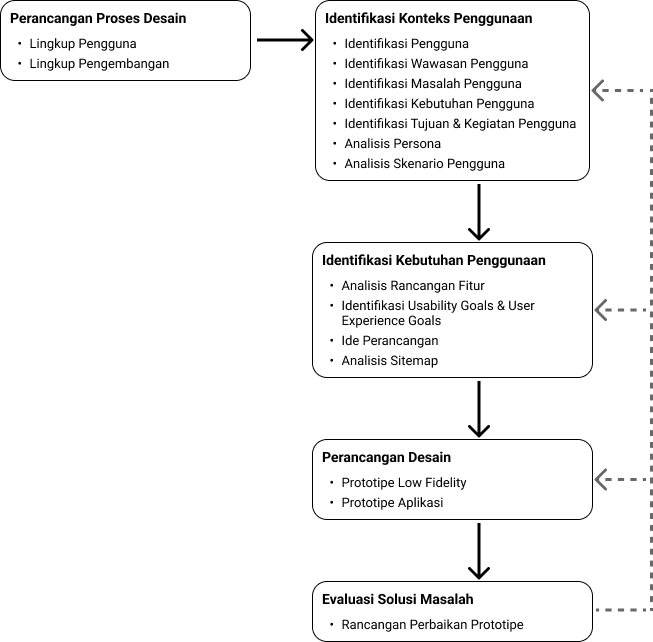
\includegraphics[width=0.8\textwidth]{chapter-3-alur-penelitian.png}
%   \caption{Alur Kerja Penelitian}
%   \label{fig:diagram_alur_kerja}
% \end{figure}

% \subsection{Perancangan Proses Desain}
% Ruang lingkup yang ditentukan pada penelitian ini adalah sebagai berikut

% \begin{enumerate}
%   \item Lingkup Pengguna
%   \subitem Target pengguna dari penelitian ini adalah masyarakat Indonesia yang pernah menggunakan atau memiliki ketertarikan terhadap aplikasi pencegah distraksi. Rentang usia dari target pengguna tidak dibatasi, namun difokuskan kepada golongan \textit{millenials} dengan rentang usia 18-30 tahun.
%   \item Lingkup Pengembangan
%   \subitem Desain interaksi aplikasi pencegah distraksi yang dibuat memiliki bentuk \textit{mobile interface} dengan mewujudkan sebuah prototipe aplikasi dalam \textit{platform Android}. Aplikasi Digital Wellbeing milik Google ditetapkan menjadi garis dasar pengembangan prototipe aplikasi tersebut.
% \end{enumerate}


% \subsection{Identifikasi Konteks Penggunaan}

% Pada tahap ini dilakukan analisis hasil riset penggunaanalisis terhadap hasil riset yang


% \subsection{Identifikasi Kebutuhan Pengguna}


% \subsection{Perancangan Desain}


% \subsection{Evaluasi Solusi Masalah}



% % Ketiga solusi yang telah diuraikan pada subbab \ref{sec:analisis_solusi} akan diimplementasikan dalam prototipe aplikasi, beserta fitur-fitur lain pada Digital Wellbeing yang akan mendukung solusi tersebut. Prototipe aplikasi ini akan diimpementasikan pada \textit{platform} Android. Secara garis besar, proses perancangan prototipe aplikasi akan menggunakan pendekatan \textit{user-centered design} (UCD).

% Seperti yang telah disebutkan pada subbab \ref{sec:metodologi}, metodologi yang digunakan dalam pengerjaan Tugas Akhir ini akan menggunakan pendekatan UCD. Dengan maksud mengikuti prosesnya, maka langkah selanjutnya yang akan dilakukan adalah mengumpulkan data. Pengumpulan data akan dilakukan dengan menyebarkan form secara online serta melakukan wawancara dengan responden yang bersedia untuk bekerja sama lebih lanjut. Proses ini akan dilaksanakan pada periode pengerjaan Tugas Akhir 2. Pengumpulan data ini bertujuan untuk melakukan validasi terhadap permasalahan yang sudah dianalisis, dan juga tidak menutup kemungkinan untuk menemukan permasalahan desain interaksi lain dari masukan pengguna.

% Setelah melakukan pengumpulan data, akan dilakukan analisis terhadap masukan yang didapat untuk mejadi kebutuhan perangkat lunak. Hasil analisis juga akan memvalidasi analisis masalah dan solusi yang didapat dari observasi penulis pada subbab \ref{sec:analisis_masalah} dan \ref{sec:analisis_solusi}.

% Kebutuhan perangkat lunak yang telah disusun akan diimplementasi dalam bentuk prototipe \textit{low-fidelity} terlebih dahulu. Setelah dilakukan evaluasi, maka implementasi akan dilanjutkan dalam bentuk prototipe \textit{high-fidelity}. Setelah menjalani evaluasi, maka perancangan prototipe aplikasi akan dikerjakan. Prototipe aplikasi diharapkan akan menghasilkan data dengan kualitas yang lebih tinggi pada saat evaluasi dibandingkan saat menggunakan prototipe \textit{low-fidelity} atau \textit{high-fidelity}. Hasil evaluasi juga akan menentukan apakah aplikasi akan menjalani proses iterasi atau diimplementasi lebih lanjut.

% \blindtext